\documentclass[ngerman]{article}
\usepackage[utf8]{inputenc}
%\usepackage[T1]{fontenc}
%\usepackage{lmodern}
\usepackage{amssymb,amsmath}
%\usepackage{ifxetex,ifluatex}

\usepackage[german]{todonotes}
\usepackage{hyperref}
\hypersetup{colorlinks,linkcolor=,urlcolor=blue}

\usepackage{csquotes}
\usepackage{paracol}
\usepackage{listings}

\usepackage{enumitem}

\usepackage{float}
\newfloat{floatquote}{tbp}{loq}
\floatname{floatquote}{Zitat}
\usepackage{caption}
\captionsetup{font = small, format = hang}

% Um Zitate zu referenzieren
%\usepackage{cleveref}
%\crefname{floatquote}{Zitat}{Zitate}
%\Crefname{floatquote}{Zitat}{Zitate}

%\hypersetup{colorlinks=true,linkcolor=,urlcolor=black}
%\hypersetup{colorlinks=false}%,linkbordercolor=red,linkcolor=green}

\usepackage{algorithm}
\usepackage{algorithmic}

% Folgende Zeilen waren im orignalen Markdown Export, ich hab sie erstmal auskommentiert.
%\setlength{\parindent}{0pt}
%\setlength{\parskip}{6pt plus 2pt minus 1pt}
%\setlength{\emergencystretch}{3em}  % prevent overfull lines
%\setcounter{secnumdepth}{0}

\title{180: Testen, Verifizieren, Analysieren}
\author{Ricarda Schüler und Stefan Bunk}
\date{24.01.2016}

\begin{document}

\listoftodos
\tableofcontents

\section{Überblick über die Anwendung}
\label{sec:ueberblick}

\paragraph{Sinn und Zweck}

180 ist eine Web-Anwendung, die Bachelor-Studenten des Hasso-Plattner-Instituts dabei unterstützt, eine korrekte Belegung zu finden, und somit ihr Bachelorstudium erfolgreich zu beenden.
Durch die Wahl von unterschiedlichen Vertiefungsgebieten sowie die Tatsache, dass viele Veranstaltungen mehreren Vertiefungsgebieten zuordenbar sind, kann es schwierig werden, eine korrekte Belegung zu finden.

Der Name 180 entstammt den 180 Leistungspunkten, die erforderlich sind, um das Bachelorstudium erfolgreich abzuschließen.
Es existiert desweiteren ein Schwesterprojekt namens 120, das von Masterstudenten des HPIs genutzt werden kann, und das den gleichen Zweck verfolgt.
Dieses Dokument befasst sich allerdings nur mit 180.

\paragraph{Entwicklungsparadigma und Programmiersprache}

Also typische Webanwendung wurde 180 in HTML, CSS und JavaScript geschrieben.
Dabei funktioniert es als rein clientseitige Anwendung, d.h. es ben"otigt keine weitere serverseitige Programmiersprache.
Es existieren keine automatisierten Tests, daher eignet sich das Projekt gut, um eine breite Testbasis in einem bestehenden Projekt aufzubauen.
Die Entwicklung folgt dem Wasserfallmodell.
Zunächst wurden die Anforderungen gesammelt, allerdings nicht formal, sondern in einer losen Liste.
Nach einer Planungsphase wurde das Projekt dann implementiert.
Nach der erfolgreichen Ver"offentlichung ist das Projekt zurzeit in der Wartungsphase.

\paragraph{Anforderungen, Spezifikation und Dokumentation}

Die Anwendungen wurde aus dem persönlichen Bedarf heraus entwickelt, und es gab keinen externen Auftraggeber.
Alleiniger Entwickler war Stefan Bunk, einer der Autoren dieses Dokuments.
Obwohl es damit keine Spezifikation im klassischen Sinne gibt, sind dennoch die zu implementierenden Regeln genau festgelegt:
In der \href{http://www.uni-potsdam.de/ambek/ambek2010/15/Seite3.pdf}{Fachspezifischen Ordnung für das Bachelor- und Masterstudium im Fach IT-Systems Engineering an der Universität Potsdam}, der Studienordnung, wird genau festgelegt, wie ein Student seinen Belegungsplan zusammenstellen muss, um den Bachelorabschluss vom HPI zu erhalten.

\begin{itemize}
    \item
        Spezification: Studienordnung des HPI -- \todo{Vorstellung Regeln, Vertiefungsgebiete}
    \item
        Vertrauliche Daten: kein Sharen über das Internet
\end{itemize}

\paragraph{Aktueller Teststatus und Bug Repositories}

Wie bereits erw"ahnt existieren keine automatisierten Tests.
Bei der Enwicklung wurde der Code wiederholt manuell getestet.

Als \href{https://github.com/knub/onehundredandeighty/issues?q=is:issue}{Bug Repository} wird die von Github bereitgestellte Funktion der \emph{Issues} verwendet.
Dort kann der Entwickler, aber auch Nutzer der Anwender, Bug-Berichte oder Feature-W"unsche abgeben, die dann eine eindeutige Nummer erhalten.
Wurde der Fehler behoben, oder entschieden, den Wunsch nicht zu implementieren, kann das Issue geschlossen werden.

Bisher wurden f"unf Issues gemeldet:
\begin{itemize}
    \item
        \href{https://github.com/knub/onehundredandeighty/issues/30}{2 Feature-Requests} nach Berechnung der Gesamtnote -- wird nicht implementiert
    \item
        \href{https://github.com/knub/onehundredandeighty/issues/20}{1 Syntaxfehler}, der die Ausführung des Programmes unmöglich machte
    \item
        \href{https://github.com/knub/onehundredandeighty/issues/4}{1 Feature-Request} nach variabler Anzahl der Semester, der teilweise umgesetzt wurde.
    \item
        \href{https://github.com/knub/onehundredandeighty/pull/5}{1 Issue} aufgrund einer Änderung der Wirtschaftsvorlesung, die statt zwei 3-LP-Veranstaltungen ab dem WS11/12 als eine 6-LP-Veranstaltung angeboten wurden.
\end{itemize}

\paragraph{Rollenverteilung der Tester}

Einer der Autoren dieses Dokumentes war der Entwickler von 180.
Beide Autoren sind bzw. waren in ihrem Bachelorstudium aktive Nutzer der Anwendung.
Im Folgenden werden beide auch noch die Rolle der Tester einnehmen.

\section{Initialer Test Plan}

\subsection{Verifikation und Validation}

\paragraph{Validation: Die richtige Anwendung bauen!}

180 wurde entwickelt unter der Annahme, dass es für jeden Studenten kompliziert ist, sein Studium entsprechend der Studienordnung zu planen.
Insbesondere die Beachtung aller Regeln der Vertiefungsgebiete ist kompliziert und erfordert mehrfaches Überprüfen aller Bedingungen.
\todo{Beispiel hinzufuegen}

%\begin{quote}
%    \begin{displayquote}
%        Das Bachelorstudium im Fach IT-Systems Engineering wird an der Universität Potsdam als Ein-Fach-Studium angeboten.
%        Es umfasst 180 LP inklusive Bachelorarbeit, Softwareprojekttätigkeit und 30 LP fachintegrativer Schlüsselqualifikationen.
%    \end{displayquote}
%    \captionof{floatquote}{Output of the Program}\label{quo1}
%\end{quote}

In diesem Bereich lässt die Studienordnung einen großen Spielraum zu, der entsprechend der eigenen Interesseren ausgefüllt werden kann aber auch muss.
Die Menge aller gültigen Belegungen ist damit sehr groß, übersieht man allerdings eine einzige Bedingung führt dies zu einem ungültigen Belegungsplan.
Merkt man dies nicht rechtzeitig, muss im schlimmsten Fall ein weiteres Semester im Bachelorstudium eingeplant werden.

Daher ist die Idee von 180 diese manuelle und fehleranfällige Prüfung zu automatisieren.
Da die Regeln der Studienordnung sich nicht schnell ändern (mehr zu möglichen Änderungen der Studienordnung weiter unten \todo{vielleicht als Footnote}), genügt es, die Regeln einmal korrekt zu implementieren.
Daher ist dies auch der zentrale Punkt der Validierung:
Die Anwendung muss genau dann ausgeben, dass ein Belegungsplan valide ist, wenn er nach den Paragraphen der Studienordnung korrekt ist.
Kann die Anwendung dies nicht garantieren, ist sie nahezu nutzlos.
Wird der Anwendung nicht vertraut, wird sie niemand nutzen, da sowieso eine manuelle Prüfung notwendig wird.

Wir beginnen mit der Validation, indem wir jeden Paragraphen der Studienordnung analysieren, und daraus zu testende Eigenschaften eines korrekten Belegungsplans ableiten.
Sind aus einem Paragraphen keine Tests ableitbar, stellen wir dies in kursiver Schrift dar.

\setlength{\parindent}{0cm}

\begin{paracol}{2}
\textbf{§~1 Geltungsbereich}
\switchcolumn
\emph{Keine Tests notwendig, lediglich Einleitung}
\\
\switchcolumn*

\textbf{§~2 Gliederung des Studiums}
\switchcolumn
Es müssen mind. 180 LP erreicht werden.
\\
\switchcolumn*

\textbf{§~3 Dauer des Studiums}
\switchcolumn
Das Studium darf nicht länger als 12 Semester dauern.
\\
\switchcolumn*

\textbf{§~4 Nachteilsausgleich}
\switchcolumn
\emph{Keine Tests notwendig}
\\
\switchcolumn*

\textbf{§~5 Abschlussgrade}
\switchcolumn
\emph{Keine Tests notwendig, lediglich akad. Titel wird vorgestellt}
\\
\switchcolumn*

\textbf{§~6 Ziel des Studiums und Berufsrelevanz}
\switchcolumn
\emph{Keine Tests notwendig, lediglich Vision des Studiums}
\\
\switchcolumn*

\textbf{§~7 Studienverwaltung; Leistungserfassungsprozess}
\switchcolumn
\emph{Keine Tests notwendig, lediglich Information über Notenvergabe}
\\
\switchcolumn*

\textbf{§~8 Freiversuche}
\switchcolumn
Prüfungen dürfen maximal dreimal wiederholt werden.
\\
\switchcolumn* 

\textbf{§~9(1) Module des Bachelorstudiums}
\switchcolumn
Die Veranstaltungen PT1\footnote{Erläuterung der Abkürzungen im Anhang}, PT2, GDS, SWA, MOD1, MOD2, SWT1, Mathe1, Mathe2, TI1, TI2 müssen belegt werden.
Das gleiche gilt für die Veranstaltungen ``Wirtschaftliche Grundlagen'' und ``Rechtliche Grundlagen''.
\\
\switchcolumn*

\textbf{§~9(2) Softwarebasissysteme}
\switchcolumn
Die Veranstaltungen BS1 muss belegt werden.
Ebenso müssen von den Veranstaltungen CG1, DBS1, POIS1, HCI1 sowie WWW mindestens drei belegt werden.
\\
\switchcolumn*

\textbf{§~9(3) Vertiefungsgebiete}
\switchcolumn
Dieser Paragraph beinhaltet die komplexen Regeln für Vertiefungsgebiete.
Dieser wird in einem Extra-Abschnitt behandelt \todo{Extra-Abschnitt}.
\\
\switchcolumn*

\textbf{§~9(4) Softskills}
\switchcolumn
Die Veranstaltung ``Projektmanagement'' muss belegt werden.
Zusätzlich müssen 6 weitere LP im Gebiet Softskills belegt werden.
\\
\switchcolumn*

\textbf{§~10 Softskills}
\switchcolumn
\emph{Keine Tests notwendig, lediglich Information über Notenvergabe}
\\
\switchcolumn*

\textbf{§~11 Softwareprojekttätigkeit}
\switchcolumn
Das Bachelorprojekt muss im Umfang von 30 LP belegt werden.
\\
\switchcolumn*

\textbf{§~12 Bachelorarbeit}
\switchcolumn
Es muss eine Bachelorarbeit im Umfang von 12 LP geschrieben werden.
\\
\switchcolumn*

\textbf{§~13 -- §~19}
\switchcolumn
\emph{Keine weiteren Tests notwendig}
\\
\switchcolumn*
\end{paracol}

\paragraph{Verifikation: Die Anwendung richtig bauen!}

Um die Anwendung richtig zu bauen, folgt man der Spezifikation.
In diesem Fall gibt es keine interne, von den Entwicklern gemeinsam mit den Anwendern festgelegte Spezifikation.
Allerdings gibt es eine externe Spezifikation: die Studienordnung.
Diese wurde zwar nicht mit dem Ziel geschrieben, als Grundlage für die Entwicklung einer Anwendung zu stehen, doch definiert sie sehr genau die Anforderungen an einen korrekten Belegungsplan.
Wir betrachen daher im Folgenden die Studienordnung als die Spezifikation für 180.
Erfüllt 180 am Ende alle Paragraphen der Studienordnung mit im Programm implementierten Regeln, ist das Programm korrekt.

Die Studienordnung ist als Artefakt sehr statisch, sie ändert sich nahezu nie.
Zusätzlich zur Studienordnung sind aber die halbjährlich erscheinenden Vorlesungsverzeichnisse relevante Artefakte für 180.
In diesen wird festgelegt, welche Veranstaltungen angeboten werden und welchen Gebieten sie zugeordnet werden können.
Damit ist die Anwendung auch niemals fertig, da diese Pflege der Daten halbjährlich vorgenommen werden muss.

In unserem Fall reicht es, die Validation einmalig durchzuführen, da sich die Studienordnung nicht ändert.
Mit der Abdeckung aller Paragraphen ist sichergestellt, dass 180 auch wirklich den Anforderungen der Studenten genügt.
Die Verifikation, u.a. die korrekte Implementierung der Regeln sowie die korrekte Aktualisierung der Semesterdaten, muss permanent durchgeführt werden.
Dies geschieht auch im Rahmen dieses Projektes, indem wir Tests entwickeln.

\subsection{Welche Technologien sollen während der Entwicklung angewandt werden?}

\begin{itemize}
    \item
        TDD
    \item
        static analysis -- bis jetzt gar nicht umgesetzt
    \item
        Randomisierte Tests bieten sich nicht an, Zuverlässigkeit am besten über genau Tests.
\end{itemize}

Laut dem ursprünglichen Paper von D. Hamlet über Random Testing.
The [..] meaning of ``random testing'' refers to an
explicit lack of ``system'' in the choice of test data, so that there is
no correlation among different tests.

In unserem Fall müssen die Testfälle aber sehr genau auspezifiert sein, um bestimmte Grenzfälle abzudecken. Eine zufällige Belegung wird nahezu immer falsch sein.

Tradeoff Kosten-Korrektheit: Bei uns ganz klar in Richtung Korrektheit.
Korrektheit ist oberstes Gut, weil eine fälschlicherweise korrekte Belegung unschöne Folgen haben kann.

Macht die Anwendung unnnutzbar, wenn man sich nicht darauf verlassen kann.

\subsection{Wann ist die Anwendung bereit für eine Veröffentlichung?}

Wir definieren Fertigkeit (``readiness'') auf Basis von drei Faktoren:

\begin{itemize}
    \item \textbf{Korrektheit}:
        Wie bereits im ersten Abschnitt erwähnt ist die Korrektheit der Anwendung das wichtigste Kriterium.
        Alle Regeln der Studienordung müssen korrekt implementiert und abgedeckt sein.
    \item \textbf{Vertraulichkeit}:
        Die Daten des Nutzers verbleiben immer auf dem lokalen Rechner und werden insbesondere nicht in einer Datenbank gespeichert.
        Der Belegungsplan eines Nutzers sollte privat bleiben und für den Betreiber des Servers niemals einsehbar sein.
    \item \textbf{Usability}:
        Die Webseite sollte gut zu benutzen sein.
        Insbesondere muss zu jedem Zeitpunkt klar sein, was die aktuelle Belegung ist, und ob diese korrekt ist oder nicht.
\end{itemize}

Von den drei Fertigkeits-Kritieren ist die Usability am schwierigsten zu erfassen, da dieses subjektive Empfinden nur über eine User-Study ermittelt werden kann.
Dies geschieht nicht im Rahmen dieses Projektes.
Bei der Vertraulichkeit geht es darum, dass wir sensibel mit den Daten des Nutzers.
Insbesondere ist wichtig, dass wir den Belegungsplan des Nutzers nicht auf dem Server speichern.
Dies erreichen wir, indem wir per Design die Daten nur auf dem Rechner des Nutzers speichern, und sie nie über das Netzwerk schicken.
Daher erfordert diese Anforderung keine expliziten Tests.

Die Korrektheit der Anwendung testen wir im folgenden Kapitel ausführlich über automatisierte Tests.
Das wir die richtigen Regeln implementieren, haben wir bereits im Abschnitt zur Validierung beschrieben.

Ein weiterer üblicherweise gewählter Faktor um die ``readiness'' zu definieren ist die Verlässlichkeit (``reliability'') der Anwendung.
Dies ist aber in unserem Fall kein Problem, weil es sich um eine statische Webseite handelt, und damit keinerlei Ressourcen des Server über das Ausliefern der Seite hinaus benötigt werden.
Desweiteren kann sich der Nutzer die Anwendung auch lokal auf seinen Rechner herunterladen, und die Anwendung so nutzen.
Selbst wenn der Nutzer auf die Online-Anwendung vertraut und diese für eine kurze Zeit nicht erreichbar ist, stellt dies auch kein Problem dar, da eine Studien- und Belegungsplanung üblicherweise über einen Zeitraum von mind. 3 Jahren erfolgt.

\subsection{Wie wird die Qualität in zukünftigen Releases sichergestellt?}

Das Hauptproblem der Aktualisierung sind die halbjährlich veröffentlichten Lehrveranstaltungsverzeichnisse.
Diese müssen manuell in 180 eingepflegt werden.
Listing~\ref{lst:data} zeigt einen Ausschnitt aus der Daten-Datei.
Hierbei ist insbesondere auf die Vertiefungsgebiete einer Veranstaltung zu achten.
Wird bei einer Veranstaltung ein falsches Vertiefungsgebiet eingetragen, macht dies eigentlich gültige Belegungen ungültig, oder erlaubt Belegungen, die nicht erlaubt werden sollten.

Da die Pflege dieser Daten manuell geschieht, ist sie sehr fehleranfällig.
In der Vergangenheit kam es bereits zu Fehlern in diesen Daten\footnote{Siehe z.B. \url{https://github.com/knub/onehundredandeighty/issues/20}}.
Solche Fälle durch Tests abzudecken ist kompliziert.

\begin{lstlisting}[caption=Ausschnitt aus \texttt{data.js},label={lst:data},frame=single]
/* .. weitere Veranstaltungen .. */
    swq: {
        kurz: "SW-Qualitaet",
        lehrform: ["Vorlesung", "Projekt"],
        modul: ["Vertiefungsgebiete"],
        semester: ["SS14", "WS15/16"],
        pflicht: false,
        empfohlen: "",
        vertiefung: ["OSIS", "SAMT"],
        cp: 6,
        vorher: [],
        dozent: ["Prof. Dr. Holger Giese"],
        nameLV: "Softwarequalitaet"
    },
/* .. weitere Veranstaltungen .. */
\end{lstlisting}


Ein offensichtliches Problem stellt die Änderung oder Neuverfassung der Studienordnung dar.
In diesem Fall muss die Anwendung entweder behutsam angepasst werden, oder komplett neu entwickelt werden.
Deswegen ist es wichtig, von einer Änderung der Studienordnung so schnell wie möglich zu erfahren.
Es lässt sich dafür aber keine gute technische Lösung implementieren.
Da Änderungen der Studienordnung aber öffentlich angekündigt werden müssen, und oft auch mit Diskussionen zwischen den Studierenden und Lehrenden einhergehen, verlassen wir uns auf schnelles Feedback des Fachschaftsrates oder der Studierendenschaft.

Technologisch sind keine Inkompatibilitäten in den nächsten Jahren zu erwarten.
180 nutzt moderne Webtechnologien wie HTML5, CSS3 und JavaScript.
Deswegen ist in den nächsten Jahren keine Inkompatibiliät oder Beendigung der Unterstützung durch Browser-Hersteller zu erwarten.

\subsection{Wie kann der Entwicklungsprozess selbst verbessert werden?}

Wie bereits erwähnt ist das Hauptproblem die Aktualisierung der Veranstaltungsdatenbank.

\begin{itemize}
    \item
        Code Reviews (insebesondere von nachträglichen Änderungen)
    \item
        2 unabhängige Änderungseingabe (neue Veranstaltung) -- erst dann in System
\end{itemize}

Vorher manuelles, fehleranfälliges Testen. Durch die von uns zu
entwickelnden Tests wird das manuelle Testen unnötig. Durch eine hohe
Testabdeckung steigt desweiteren

\subsection{Klassifizierung nach verschiedenen Test-Kriterien}


\subsection{Zusammenfassung}
\label{sec:zusammenfassung}

Im Folgenden fassen wir zusammen, wie wir den Status quo durch unseren initialen Test-Plan verbessern möchten.

\begin{itemize}
    \item Mapping zwischen Regeln und Paragraphen, zeigen dass vollständig (Validation-Testing)
    \item
        Defekt-Testing: Hier werden wir ein Test-Skript entwickeln, dass die data.js, die schon mehrfach Syntax-Fehler enthielt, auf ebendiese überprueft
    \item
        Unit-Tests für jede Regel im Programm
    \item
        System-Tests mit kompletten, echten Belegungsplänen
    \item
        Kleine User-Study mit folgenden Fragen: ** dfasdf ** dfasdf
\end{itemize}

\todo{Development, Release, Uesrtesting (wir haben nur das erste)}
\todo{Unit/Component, Integration, System Testing}

\section{Testing}

In diesem Kapitel werden Beispiele für verschiedene Testarten dargestellt. Dabei wurde versucht die Anwendung in die breite hin zu testen. Das heißt für die verschiedenen Ansätze wurde jeweils eine Funktion von 180 herausgenommen. In den meisten Fällen gibt es weitere Programmteile, welche genau so getestet werden können. Es geht in diesem Abschnitt aber viel mehr darum, einen Überblick zu geben, was überhaupt möglich ist.
GUI-Testing haben wir in diesem Abschnitt erst einmal nicht betrachtet, sondern uns auf die Logik im Hintergrund konzentriert.

\subsection{Graph Coverage}
\todo{warum hilft graph coverage tests die testplanziele zu erfüllen (bzw. teilweise)}
\subsubsection{Control Flow Graph}
Es gibt die sogenannte Time Rule. Diese prüft, ob eine bestimmte Lehrveranstaltung in einem bestimmten Semester angeboten wurde beziehungsweise wahrscheinlich angeboten wird. Der Algorithmus zur Prüfung ist in Pseudocode in Algorithmus \ref{algo:time_rule} dargestellt. Der daraus resultierende Graph ist in Abbildung \ref{Fig:graph_time_rule} zu sehen.


\begin{algorithm}[h!]
\caption{Time Rule}
\label{algo:time_rule}
\algsetup{indent=2em}
\begin{algorithmic}[1]
    \REQUIRE 1 Course
    \ENSURE Boolean (offered in this semester)
    \STATE semester = getSemester(course)


    \IF{course chosen}
        \RETURN true
    \ELSE
        \IF{Semester is in past}
            \RETURN course offered in semester?
        \ELSE 
            \IF{semester is Sommersemester}
                \RETURN course offered in this semester or offered in past sommersemester
            \ELSE
                \IF{semester is Wintersemester}
                    \RETURN course offered in this semester or offered in past Wintersemester 
                \ELSE 
                    \RETURN Error
                \ENDIF
            \ENDIF
       \ENDIF
   \ENDIF
\end{algorithmic}
\end{algorithm}


\begin{figure}[h!]
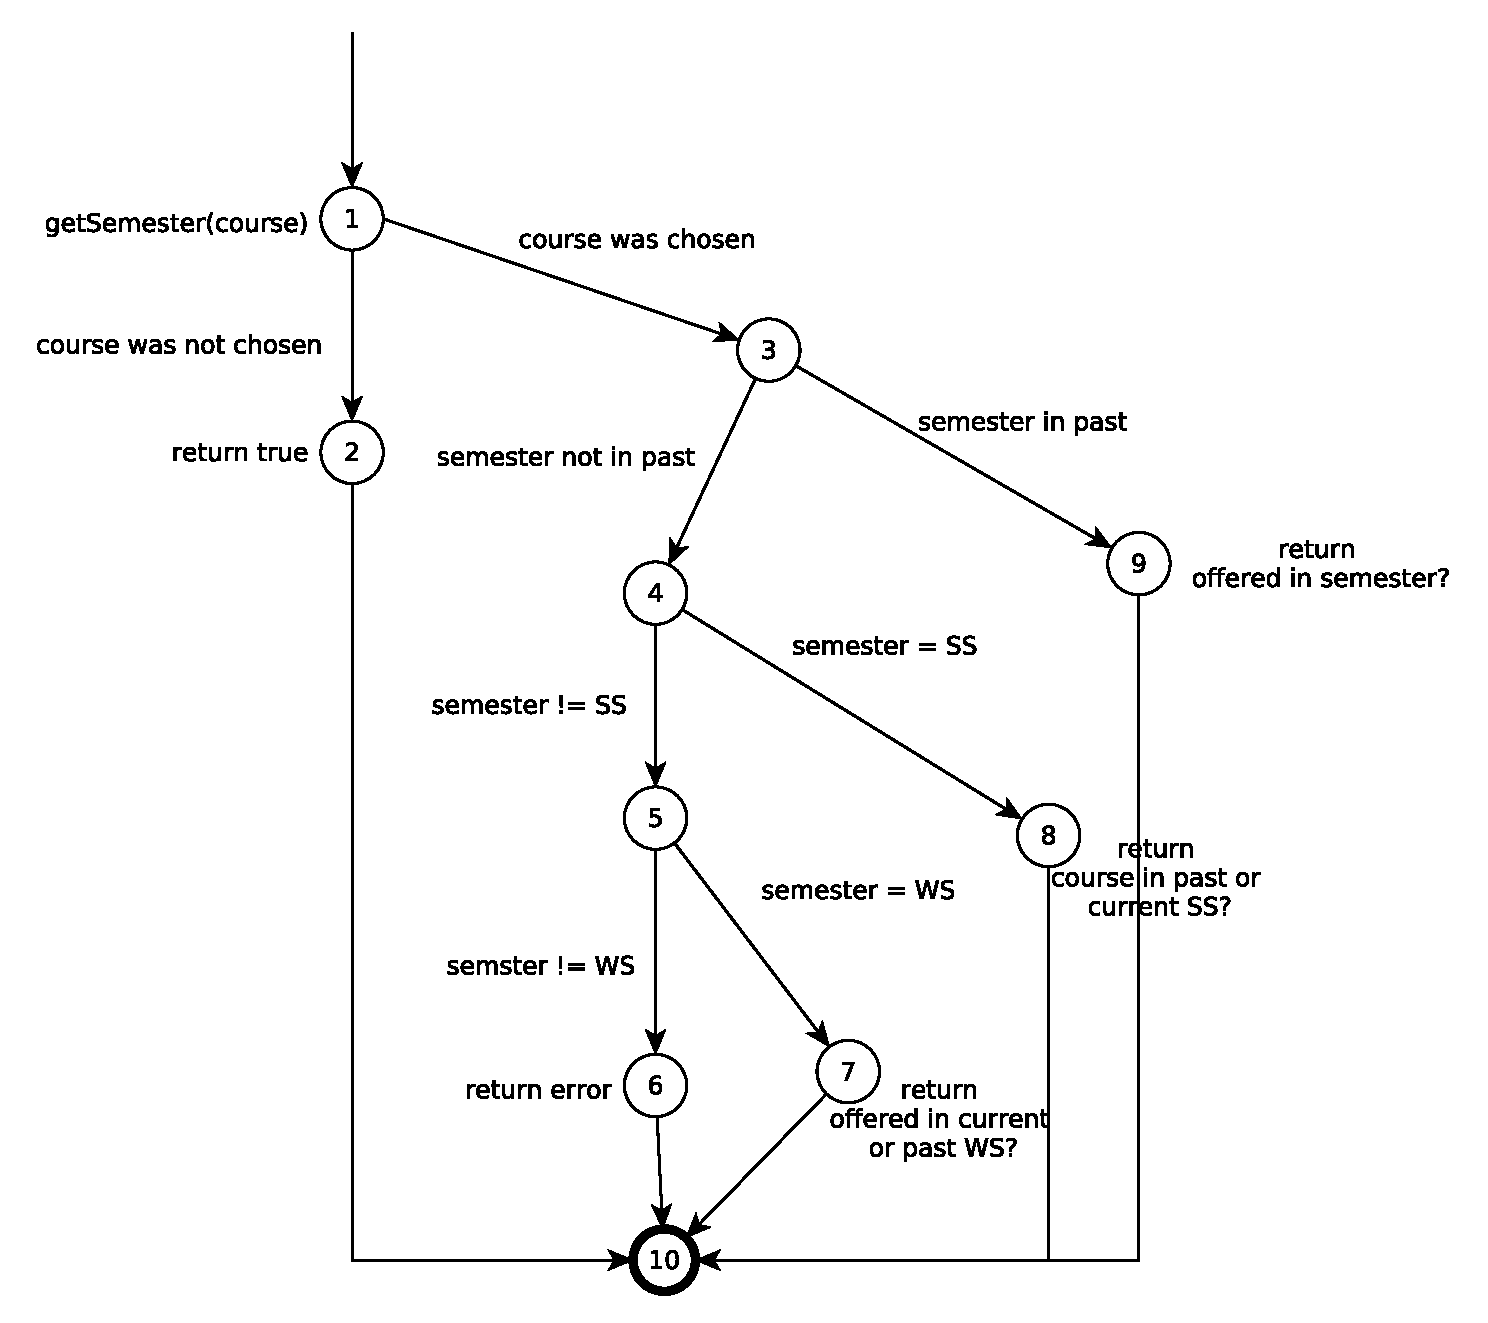
\includegraphics[width=0.8\textwidth]{figures/time_rule.pdf}
\caption{Graph der Time Rule}
\label{Fig:graph_time_rule}
\end{figure}

Wir möchten Edge-Pair-Coverage für diese Regel erreichen, da damit alle Fälle abgedeckt sind. 
Dazu müssen Kanten-Kanten-Kombinationen in der Testsuit enthalten sein.
Nachfolgend sind alle Test Requirements und Testpfade abgebildet. Die Testpfade, welche zusammen alle Fälle abdecken, wurden mit automatistierten Tests umgesetzt \footnote{Tests siehe \url{https://github.com/knub/onehundredandeighty/blob/testing/test/cfg_test.js}}.


\vspace{1em}


\begin{paracol}{2}
 \textbf{Test Requirement}
\begin{enumerate}[label=\Alph*]
\item $\lbrack 1,2,10 \rbrack$
\item $\lbrack 1,3,4\rbrack$
\item $\lbrack 1,3,9\rbrack$
\item $\lbrack 3,4,5\rbrack$
\item $\lbrack 3,4,8\rbrack$
\item $\lbrack 3,9,10\rbrack$
\item $\lbrack 4,5,6\rbrack$
\item $\lbrack 4,5,7\rbrack$
\item $\lbrack 4,8,10\rbrack$
\item $\lbrack 5,6,10\rbrack$
\item $\lbrack 5,7,10\rbrack$
\end{enumerate}

\switchcolumn
\paragraph{Test Paths}
\begin{enumerate}[label=(\roman*)]
\item $\lbrack 1, 2, 10 \rbrack$
\item $\lbrack 1, 3, 4, 5, 6, 10\rbrack$
\item $\lbrack 1, 3, 4, 5, 6, 7, 10\rbrack$
\item $\lbrack 1, 3, 4, 8, 10\rbrack$
\item $\lbrack 1, 3, 9, 10\rbrack$
\end{enumerate}

\begin{table}
\begin{tabular}{|l|p{2.5cm}|}
\hline
\textbf{Test Pfade} & \textbf{Abgedeckte TR} \\ \hline \hline
(i) & A\\ \hline
(ii)  & B, D, G, J \\ \hline
(iii) & B, D, H, K\\ \hline
(iv) & B, E, I\\ \hline
(v) & C, F\\ \hline \hline
Coverage & A, B, C, D, E, F, G, H, I, J, K, H\\ \hline
\end{tabular}
\end{table}

\end{paracol}

\subsubsection{Finite State Machines}
Veranstaltungsstatus: gewählt, wählbar, gefiltert...


\subsubsection{Use Cases}
Für \emph{Onehundredandeighty} haben wir die folgenden Use Cases ermittelt:

\begin{itemize}
    \item Semester wählen
    \item Semesteranzahl verändern
    \item Belegung wählen
    \item Prüfung validieren
    \item Filtern nach verfügbaren Kursen
\end{itemize}

Für eine genaue Prüfung haben wir uns den Use Case "Belegung wählen" heraus gesucht. Dieser Use Case ist ein sehr zentraler Bestandteil der Anwendung, welcher für den Nutzer eine relativ hohe Komplexität aufweist. In Abbildung \ref{fig:aktivity_belegung_waehlen} ist das Aktivitätsdiagram dargestellt. Dieses Aktivitätsdiagram interpretieren wir nun als Graph, welcher in Abbildung \ref{fig:graph_belegung_waehlen}.

\begin{figure}[h!]
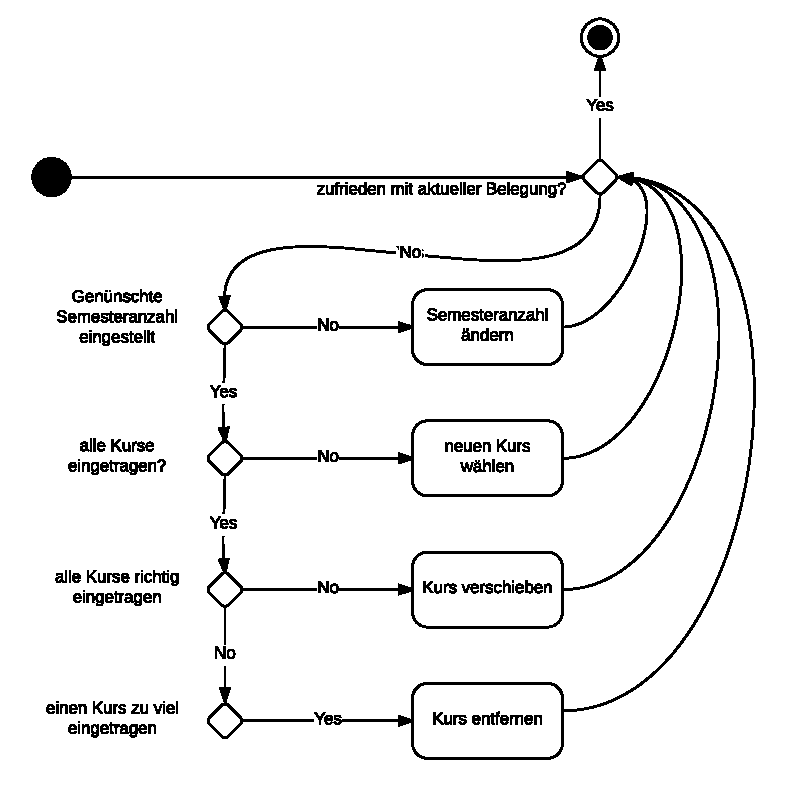
\includegraphics[width=0.8\textwidth]{figures/180_Belegungaendern_aktivitaet.pdf}
\caption{Aktivitätsdiagram vom Use Case Belegung wählen}
\label{fig:aktivity_belegung_waehlen}
\end{figure}

\begin{figure}[h!]
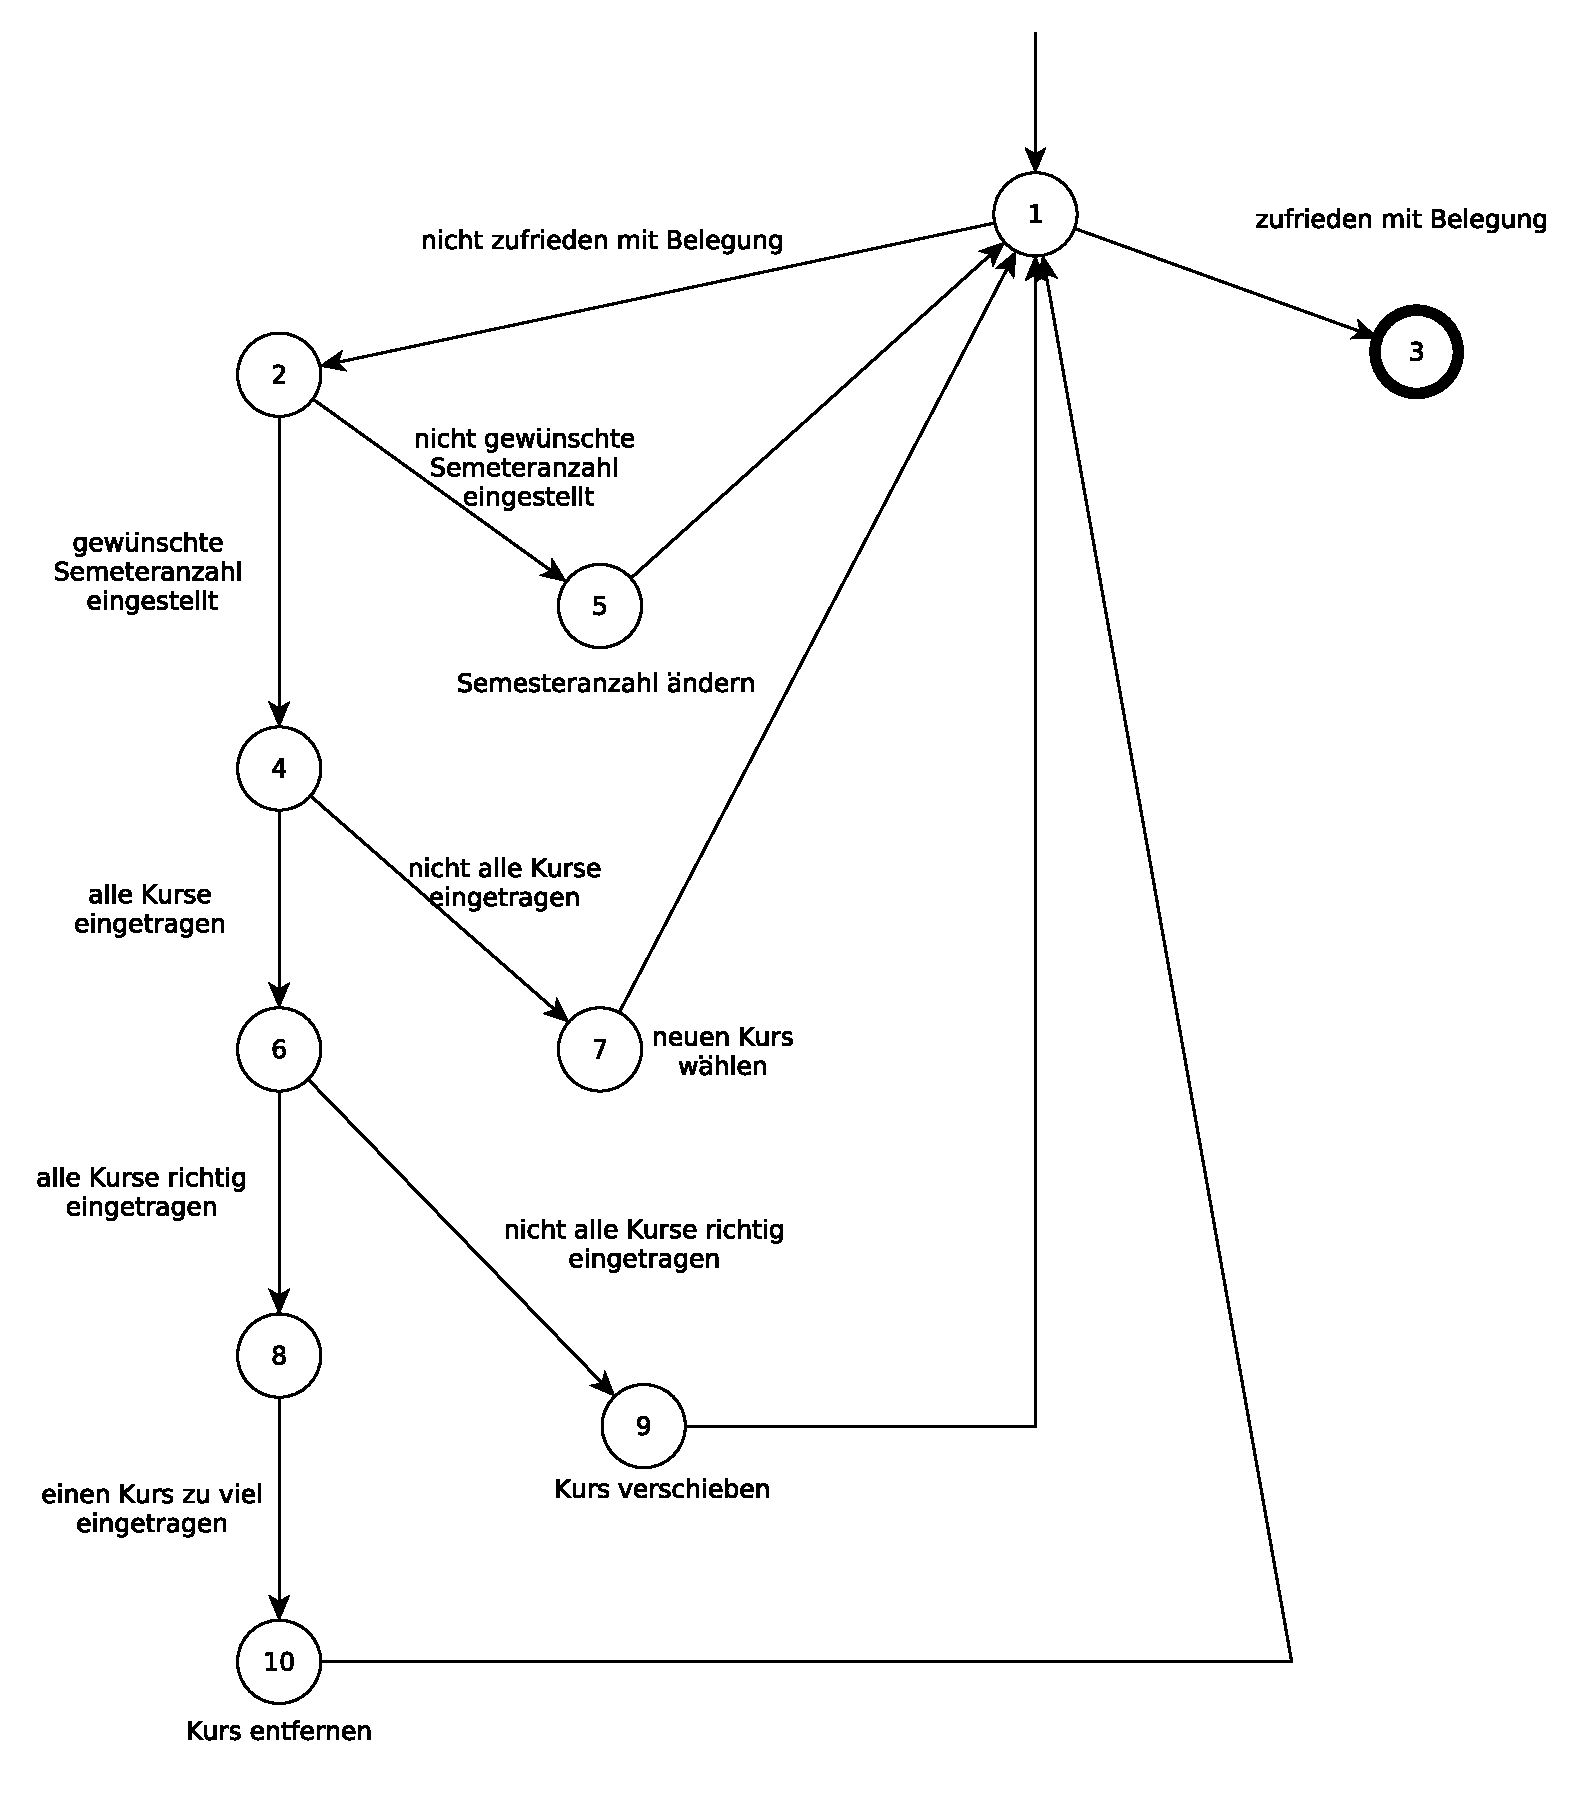
\includegraphics[width=0.8\textwidth]{figures/belegung_waehlen_use_case.pdf}
\caption{Graph vom Use Case Belegung wählen}
\label{fig:graph_belegung_waehlen}
\end{figure}

In diesem Use Case ist es theoretisch möglich, dass ein Nutzer alle einzelnen Teile oder auch eine Auswahl davon benutzt. Im Regenfall werden die Nutzer mit einem Plan herum spielen und alle einzelnen Aktionen ausführen.
Daher werden wir einen Testfall aufstellen, welcher alle Kanten und alle Knoten des Graphens mindestens einmal ausführt: 1, 2, 5, 1, 2, 4, 7, 1, 2, 4, 6, 9, 1, 2, 4, 8, 10, 1, 3


\subsection{Logik Coverage}

\subsubsection{Regel für Wirtschaftliche Grundlagen}

Die Veranstaltung Wirtschaftliche Grundlagen wurde traditionell als zwei Veranstaltungen mit jeweils 3LP durchgeführt.
Zum Wintersemester WS13/14 wurde dies geäendert, und die Veranstaltung wurde fortan als eine Veranstaltung mit 6LP angeboten.
Da 180 unabhängig vom Jahrgang funktionieren soll, gibt es daher zwei mögliche gültige Belegungen: entweder man belegt beide 3LP Veranstaltungen oder eine 6LP Veranstaltung.
Die entsprechende Bedingung ist in Listing~\ref{lst:wirtschaft} zu sehen.

Wir wollen im Folgenden diese Regel mit \emph{Correlated Active Clause Coverage (CaCC)} abdecken.
Wir wissen, dass man in einem solchen auch einfach \emph{Combinatorial Coverage} durchführen kann, indem man alle $2^n = 2^3 = 8$ mögliche Belegungen manuell prüft.
Wir werden allerdings hier zur Übung dennoch \emph{CaCC} testen.
Vereinfacht stellen wir die Formel als $(a \land b) \lor c$ dar.
\begin{lstlisting}[caption=Wirtschafts-Regel,label={lst:wirtschaft},frame=single]
return (selectedWirtschaftI && selectedWirtschaftII) ||
        selectedWirtschaftI_II;
\end{lstlisting}

\begin{table}[h!]
\begin{tabular}{|l|l|l|l|l|l|l|l|}
\hline
\textbf{Row \#} & \textbf{a} & \textbf{b} & \textbf{c} & \textbf{P} & \textbf{$P_a$} & \textbf{$P_b$} & \textbf{$P_c$} \\
\hline \hline
 1              & T          & T          & T          & \textbf{T} &                &                &                \\
 2              & T          & T          & F          & \textbf{T} & T              &   T            &                \\
 3              & T          & F          & T          & \textbf{T} &                &                & T              \\
 4              & T          & F          & F          & \textbf{F} &                &   T            & T              \\
 5              & F          & T          & T          & \textbf{T} &                &                & T              \\
 6              & F          & T          & F          & \textbf{F} & T              &                & T              \\
 7              & F          & F          & T          & \textbf{T} &                &                & T              \\
 8              & F          & F          & F          & \textbf{F} &                &                & T              \\
 \hline
\end{tabular}
\caption{Wahrheitstabelle für Wirtschaftsregel}
\end{table}

Es ergeben sich folgende Fälle, in denen die Variablen jeweils aktiv werden:
\begin{align}
    P_a &= \{ (2, 6) \} \\
    P_b &= \{ (2, 4) \} \\
    P_c &= \{ 3, 5, 7 \} \times \{ 4, 6, 8 \}
\end{align}
Mit den Test Paths $TP = \{ 2, 3, 4, 6 \}$ decken wir alle Klauseln ab\footnote{Tests siehe \url{https://github.com/knub/onehundredandeighty/blob/testing/test/wirtschafts_rule_coverage.js}}.
Dies ist gleichzeitig auch die kleinste Menge die \emph{CaCC} erreicht.

\subsubsection{Regeln für Vertiefungsgebiete}

Die Regeln für Vertiefungsgebiete sind der komplizierteste Teil der Studienordnung.
\begin{quote}
    \begin{displayquote}
Die Modulgruppen ``Vertiefungsgebiet 1'' (VT1) und ``Vertiefungsgebiet 2'' (VT2) verfolgen die vertiefende Beschäftigung mit fachwissenschaftliche Themen des IT-Systems Engineering.
Es werden die folgenden Vertiefungsgebiete angeboten:
\begin{itemize}
    \item \emph{BPET}: Business Process \& Enterprise Technologies
    \item \emph{HCT}: Human Computer Interaction \& Computer Graphics Technology
    \item \emph{IST}: Internet \& Security Technology
    \item \emph{OSIS}: Operating Systems \& Information Systems Technology
    \item \emph{SAMT}: Software Architecture \& Modeling Technology
\end{itemize}
Es sind Module in zwei Vertiefungsgebieten in einem Gesamtumfang von 24 LP zu absolvieren, wobei in VT1
bzw. VT2 jeweils mindestens 9 LP zu erbringen sind. In VT1 und VT2 müssen mindestens je eine Vorlesung
(VT1-V und VT2-V) im Umfang von 6 LP erbracht werden. Weiter müssen ergänzende Lehrveranstaltungen
(VT1-E, VT2-E, VT1/2-E) im Umfang von 12 LP absolviert werden, die sich auf beide Vertiefungsgebiete in
den möglichen Kombinationen 3+9 LP, 6+6 LP oder 9+3 LP verteilen. 
    \end{displayquote}
    \captionof{floatquote}{§~9 (3) der Studienordnung}
    \label{quo:vertiefungsgebiete}
\end{quote}

\subsection{Input}
Der Input kann von Methoden, Modulen und dem ganzen System getestet werden. Das System hat als Input ganze Belegungspläne. Diese sind sehr verschienen und können sehr komplex ausfallen. Diese werden hier nicht weiter betrachtet. 
Es gibt in 180 Helfermethoden, welche in vielen Programmteilen benötigt werden. Eine Methode ist die \emph{cartesianProduct}-Methode, welche das kartesische Produkt zweier Mengen berechnet. 
Für diese Methode werden wir beispielhaft den Input testen.

Als Eingabe werden 2 Arrays erwartet, welche jeweils eine Menge darstellen.

Wir haben uns für eine Partitionierung nach der Größe der Inputarrays entschieden. Dabei haben wir versucht die Randfälle wie keine Elemente oder nur 1 Element eine Partition zu widmen, da diese oftmals die Fehler führen. Im folgenden sind alle Partintionen dargestellt, wobei \emph{$|A1|$} die Größe vom ersten Inputarray und \emph{$|A2|$} die Größe vom zweiten Inputarray darstellt.
\begin{itemize}
\item $|A1|$ undefined und $|A2|$ undefined
\item $|A1| \geq$ 0 und $|A2|$ = undefined
\item $|A1|$ undefined und $|A2| \geq$ 0
\item $|A1|$ = 0 und $|A2|$ = 0
\item $|A1|$ = 1 und $|A2|$ = 0
\item $|A1| \geq$ 2 und $|A2|$ = 0
\item $|A1|$ = 0 und $|A2|$ = 1
\item $|A1|$ = 1 und $|A2|$ = 1
\item $|A1| \geq$ 2 und $|A2|$ = 1
\item $|A1|$ = 0 und $|A2| \geq$ 2
\item $|A1|$ = 1 und $|A2| \geq$  2
\item $|A1| \geq 2$ und $|A2| \geq $ 2
\end{itemize}

Diese Partitionierung erfüllt die Kriterien für eine gültige Partitionierung zum Inputtesten, in dem sie paarweise disjunkt sind und zusammen alle möglichen Eingaben der Methode abbilden.

Andere Partitionierungen, wie zum Beispiel die Reihenfolge der Elemente haben wir nicht als sinnvoll erachtet, da ins besondere die Reihenfolge überhaupt keine Rolle spielt.

Die entsprechenden Tests für ein Beispiel aus jeder Partition wurden implementiert \footnote{https://github.com/knub/onehundredandeighty/blob/testing/test/input.js}.



\subsection{Mutation Coverage}
Wir haben mit Hilfe von \emph{grunt-mutation-testing} \footnote{https://www.npmjs.com/package/grunt-mutation-testing} die Mutation Coverage der von uns geschriebenen Tests ermittelt.
Dabei haben wurde die Coverage von 0\% auf x\% gesteigert. Es wurden alle möglichen Mutationsarten angewandt. Dabei kann man sehen, dass einige Methoden schon fast vollständig abgedeckt sind, andere Methoden hingegen noch gar nicht getestet werden. In vielen Methoden sind einzelne Vergleiche (z.B. $<$ kann mit $\leq$ ersetzt werden) nicht vollständing abgedeckt. Bei vielen der Vergleichen ist die gleich Beziehung allerdings auch kaum relevant.



\section{Statische Analyse}

Bisher wurden nur bei neuen Pull-Requests manuelle Inspektionen durchgeführt. Dies hat allerdings auch schon mehrfach du Syntaxfehlern in zum Beispiel der oft aktualisierten Datendatei, data.js, geführt. Umso wichtiger ist es automatische statische Analyse zu benutzen.

focus auf wie asa testing unterstützt und wie testing asa unterstützt
statische analyse nicht nur code basiert, sondern auch spezifikation/dokumentation

jshint: 60 warnings
google code closure compiler: compiled code zu effizienteren code und überprüft dabei auf verschiedene sachen:
 ERROR - Parse error. IE8 (and below) will parse trailing commas in array and object literals incorrectly. If you are targeting newer versions of JS, set the appropriate language in option.
	message: "Die Vorlesung 'Wirtschaftliche Grundlagen' muss besucht werden.",
	
	mit höherer Sprache keine probleme

\end{document}
